
%%%%%%%%%%%%%%%%%%%%%%% file typeinst.tex %%%%%%%%%%%%%%%%%%%%%%%%%
%
% This is the LaTeX source for the instructions to authors using
% the LaTeX document class 'llncs.cls' for contributions to
% the Lecture Notes in Computer Sciences series.
% http://www.springer.com/lncs       Springer Heidelberg 2006/05/04
%
% It may be used as a template for your own input - copy it
% to a new file with a new name and use it as the basis
% for your article.
%
% NB: the document class 'llncs' has its own and detailed documentation, see
% ftp://ftp.springer.de/data/pubftp/pub/tex/latex/llncs/latex2e/llncsdoc.pdf
%
%%%%%%%%%%%%%%%%%%%%%%%%%%%%%%%%%%%%%%%%%%%%%%%%%%%%%%%%%%%%%%%%%%%


\documentclass[runningheads,a4paper]{llncs}

\usepackage{amssymb, amsmath}
\setcounter{tocdepth}{3}
\usepackage{graphicx}


\usepackage{url}
\urldef{\mailsa}\path|9erthaion6@gmail.com, zaxarovyn@rambler.ru|
\newcommand{\keywords}[1]{\par\addvspace\baselineskip
\noindent\keywordname\enspace\ignorespaces#1}

\begin{document}

\mainmatter  % start of an individual contribution

% first the title is needed
\title{Numerical modeling of artificial heart valve}

% a short form should be given in case it is too long for the running head

% the name(s) of the author(s) follow(s) next
%
% NB: Chinese authors should write their first names(s) in front of
% their surnames. This ensures that the names appear correctly in
% the running heads and the author index.
%
\author{Dmitriy Dolgov \and Yury Zakharov}
%
\authorrunning{CITech-2015, Almaty, Kazakhstan, 2015 September 24-27}
% (feature abused for this document to repeat the title also on left hand pages)

% the affiliations are given next; don't give your e-mail address
% unless you accept that it will be published
\institute{Kemerovo State University,\\
Kemerovo, Russia\\
\mailsa}

%
% NB: a more complex sample for affiliations and the mapping to the
% corresponding authors can be found in the file "llncs.dem"
% (search for the string "\mainmatter" where a contribution starts).
% "llncs.dem" accompanies the document class "llncs.cls".
%

\toctitle{Lecture Notes in Computer Science}
\tocauthor{Authors' Instructions}
\maketitle


\begin{abstract}
    The paper is dedicated to the mathematical model describing dynamics of
    an artificial heart valve being moved by inhomogeneous incompressible fluid flow
    with variable viscosity, and its computational method. The modeling results of
    tricuspid valve performance are presented.
\keywords{viscous inhomogeneous fluid, artificial heart valve, immersed boundary method}
\end{abstract}


\section{Introduction}
The importance of medical researches of human blood circulatory system can hardly be overestimated,
because this kind of knowledge is extremely practical and significant. Annually approximately 250 000
surgeries are performed in the world to restore or replace damaged heart valves \cite{yoganathan}, and the
quantity is expected to increase \cite{yacoub}. The solution of scientific and technical problems of the artificial valves 
creation depends on correct understanding of the interaction between blood flow and valve leaflets. Mathematical modeling
of artificial heart valves performance enables to get thorough understanding of its internal processes in order to improve its design.
There are many researches devoted to the mathematical and numerical modeling
of heart valve performance, based on which two main problem solution approaches were defined.

First approach is related to the finite element methods (\cite{taylor}, \cite{zhang}, \cite{black}). They enable to take into consideration
the complex geometry of heart, bu the necessity to take into account the interaction between fluid and flexible walls
requires constant rebuilding of the computational grid to meet the changing geometry of the object of research.
It appears to be time and computational resources consuming.

(The second approach, which is related to the immersed boundary method, is under discussion in this paper (\cite{pescin_1977},
\cite{boyce_2011}, \cite{ma_x_2013}, \cite{pilhwa_2010}). It can be used for the problems with complex geometry, and it doesn't
require grid modification.

There are various improvements of this method, in order to model more and more complex problems. In the research \cite{fai_2013}
a formulation of this method was proposed for the three dimensional flow problem of two non mixed (separated by flexible barriers)
fluids of different viscosity and density. In the papers \cite{jian}, \cite{lee} this method application in case of the two dimensional 
problem of two component fluid flow is presented.

We propose to describe the blood flow in the flexible large blood vessels and the artificial heart valve as a three dimensional
nonstationary flow of viscous incompressible fluid with variable viscosity and density (see \cite{gummel}, \cite{geidarov},
\cite{milosevic}, \cite{dolgov}). Thus, the goal of this work is to develop a mathematical model and a solution method of the problem
of artificial heart leaflet dynamics inside a blood vessel taking into account the inhomogeneous structure of the blood, and 
admixture (formed elements) circulation inside a blood vessel.

\section{Formulation of the problem}

We consider a nonstationary problem of blood flow inside a vessel with a valve. Blood consists of plasma and formed elements, which are approximately
45\% of the entire volume \cite{caro}. Vessel walls and valve leaflets consist of a large number of thin collagen fibers, they are flexible
and can change their form depending on the fluid flow. For example, the tricuspid aortic valve, lies between the left ventricle and the aorta, and 
prevents blood backflow (see Fig. \ref{fig:aortic_valve_example}):

\begin{figure}
\centering
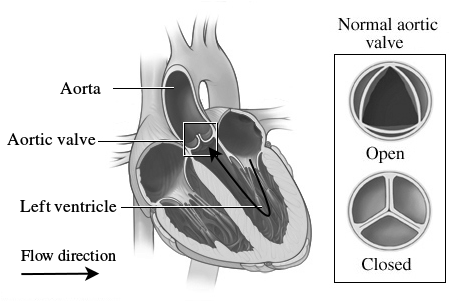
\includegraphics[height=6.2cm]{images/aorta_scheme_gray.png}
\caption{Aortic valve and its location inside heart}
\label{fig:aortic_valve_example}
\end{figure}

We model the blood as a viscous incompressible inhomogeneous two component fluid with variable viscosity, and vessel wall and valve leaflets as a
fluid impermeable surface with specified stiffness. Vessel and valve leaflets are deformed under the fluid pressure.

\begin{figure}
\centering
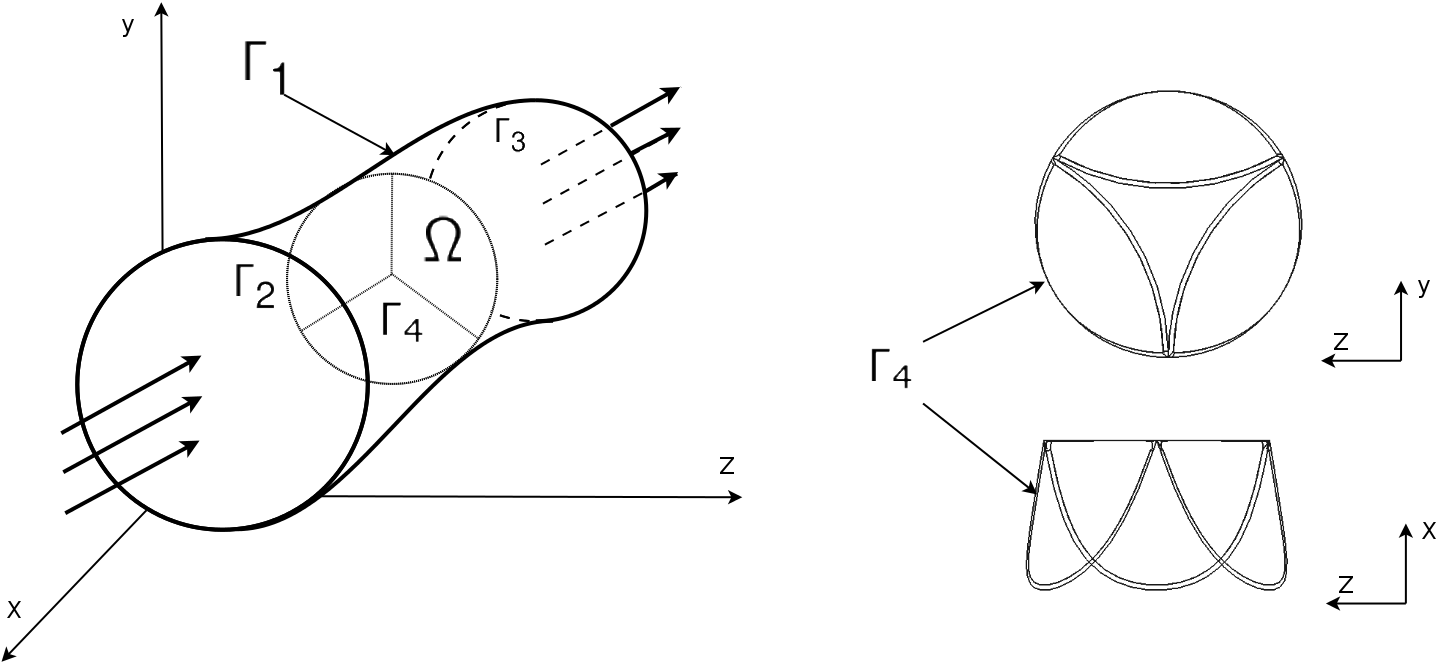
\includegraphics[width=12.5cm]{images/area_3d.png}
\caption{Computational domain boundaries}
\label{fig:area_3d}
\end{figure}

Since blood circulates through vessels under the pressure created by cardiac beats then the problem of the blood flow
can be described by Navier-Stokes nonstationary system of differential equations \cite{gummel}:
\begin{gather}
    \label{eq:navier_stokes:motion}
    \frac{\partial \vec{u}}{\partial t} + (\vec{u} \cdot \nabla) \vec{u} = - \frac{1}{\rho} \nabla p + \nabla \sigma + \vec{f}\\
    \label{eq:navier_stokes:continuity}
    \frac{\partial \rho}{\partial t} + \nabla \cdot (\rho \vec{u}) = 0 
\end{gather}

with the initial and boundary conditions:
\begin{gather}
    \label{eq:navier_stokes:velocity_conditions}
    \vec{u}(\bar{x}, 0) = \vec{u}_0 \qquad \vec{u}|_{\Gamma_1, \Gamma_4} = \vec{u}_b \qquad u_{\Gamma_2, \Gamma3} = 0\\
    \label{eq:navier_stokes:pressure_conditions}
    p_{\Gamma_2} = p_{in} \qquad p_{\Gamma_3} = p_{out}
\end{gather}

where $\bar{x}=(x,y,z) \in \Omega$, $\vec{u}=(u,v,w)$ - velocity vector, $\vec{u}_b$ - velocity of the vessel walls and valve leaflets motion under deformation,
$\rho=\rho(\bar{x}, t)$ - density, $p=p(\bar{x}, t)$ - pressure, $\sigma = \mu (\nabla \vec{u} + (\nabla \vec{u})^T)$ - viscous stress tensor,
$\mu = \mu(\bar{x}, t)$ - fluid viscosity, $\vec{f} = \vec{f}(\bar{x}, t)$ - body forces vector, which is further used to determine form of the vessel and valve leaflets.
Domain $\Omega$ is a vessel with boundary $\Gamma = \Gamma_1 \cup \Gamma_2 \cup \Gamma_3 \cup \Gamma_4$, where $\Gamma_1$ - blood vessel wall,
$\Gamma_2$ and $\Gamma_3$ - inflow and outflow domains, $\Gamma_4$ - valve leaflets (see Fig. \ref{fig:area_3d}).
As shown in \cite{ragulin}, the problem (\ref{eq:navier_stokes:motion}) - (\ref{eq:navier_stokes:continuity}) has a unique solution.

Density $\rho$ and viscosity $\mu$ are defined by following relations \cite{gummel}:
\begin{gather}
    \label{eq:viscosity}
    \mu = c (\mu_2 - \mu_1) + \mu_1\\
    \label{eq:density}
    \rho = c (\rho_2 - \rho_1) + \rho_1
\end{gather}

where $\rho_1$, $\mu_1$ - fluid density and viscosity (plasma), $\rho_2$, $\mu_2$ - admixture density and viscosity (formed elements), $c$ - admixture concentration.
Admixture concentration $c=c(\bar{x}, t)$, $c \in [0, 1]$ is determined as a solution of equation:
\begin{gather}
    \label{eq:convection}
    \frac{\partial c}{\partial t} + \vec{u} \cdot \nabla c = 0
\end{gather}

with initial conditions:
\begin{gather}
    \label{eq:convection:conditions}
    c(\bar{x}, 0) = c_0(\bar{x}), \bar{x} \in \Omega
\end{gather}

and boundary conditions at the inflow boundary:
\begin{gather}
    \label{eq:convection:conditions}
    c(\bar{x}, t)|_{\Gamma_2} = c_s(\bar{x}, t)
\end{gather}

where $c_0, c_s$ are specified functions.

One of the issues determined for this kind of problem computational solutions is the lack of one component of velocity vector in the inflow-outflow areas.
It can be solved by using the original equations (\ref{eq:navier_stokes:motion}) - (\ref{eq:navier_stokes:pressure_conditions}) at the boundaries
$\Gamma_2$, $\Gamma_3$ to determine the missing components of the velocity vector (see details \cite{gummel}).

Motion of the vessel walls and valve leaflets is defined by the forces, which return them to the original position. Valve leaflets can be deformated much more,
than vessel walls. To describe the forces, arising due to the valve deformation, the following formula is used:

\begin{gather}
    \label{eq:boundary_force}
    F = \frac{\partial}{\partial s} (T \tau) + \frac{\partial^2}{\partial s^2} (E \cdot I \frac{\partial^2}{\partial s^2} X)
\end{gather}

where $\bar{q} = (q, r, s) \in \Gamma_4$, $X(\bar{q})$ - function for describing the valve leaflets surface at the moment $t$, the coordinates $q, r, s$ are chosen 
so that the surface $X$ is presented by the large amount of parametric lines $s \rightarrow X(q^0, r^0, s)$, $T$ - tension,
that arises due to the stretching along $s$, $E$ - Young's modulus, $I$ - cross-sectional moment of inertia (see \cite{boyce_2011}, \cite{pescin_2002}).
Physically the formula above means, that the valve leaflets resist stretching, (it's related to the first term with $T$,
which is dependent on stiffness coefficient $k$), and bending (it's related to the second term, where $E$ and $I$ are referred as a stiffness coefficient $k_b$).
Formula (\ref{eq:boundary_force}) allows taking into account any changes of the valve shape.

To compute the forces, arising due to the deformation of the vessel, another formula is used, which allows taking into account only small shape changes:

\begin{gather}
    \label{eq:boundary_force_simple}
    F = k \|X - X_0\|
\end{gather}

where $\bar{q} = (q, r, s, t) \in \Gamma_1$, $X(\bar{q}, t)$, $X_0(\bar{q}, 0)$ - functions for describing the surface of vessel walls at the moment $t$ and at the initial time, $k$ - stiffness coefficient.

Researches \cite{pescin_1977}, \cite{boyce_2011} show, that in order to the interaction between vessel walls, valve leaflets and the fluid flow it is necessary
to compute the field of external body forces $f$ in the Navier-Stokes equation, based on the force $F$, and determine the current form $X(\bar{q}, t)$ 
of the vessel and the valve, based on the fluid field of velocities $\vec{u}(\bar{x}, t)$. The following equations are used for this purpose:
\begin{gather}
    \label{eq:interaction:velocity}
    \frac{\partial X}{\partial t}(\bar{q}, t) = \int_{\Omega} \vec{u}(\bar{x}, t) \cdot \delta (x - X(\bar{q}, t))\; dx\; dy\; dz\\
    \label{eq:interaction:force}
    \vec{f}(\bar{x}, t) = \int_{\Gamma} \vec{F}(\bar{q}, t) \cdot \delta (x - X(\bar{q}, t))\; dq\; dr\; ds
\end{gather}

where $\bar{q} = (q, r, s) \in \Gamma$ - point at the vessel wall or valve leaflet, $X = X(\bar{q}, t)$ - function for describing the vessel
and valve surfaces at the moment $t$, $F = F(\bar{q}, t)$ - the force of deformation resistance at given point,
$\vec{u}(\bar{x}, t)$ - fluid flow velocity vector, $\vec{f}(\bar{x}, t)$ - body forces vector, $\delta$ - Dirac delta function.

Thus the model describing the motion of the viscous inhomogeneous incompressible fluid inside vessel with valve is built. This model enables to determine
the fluid state and the surface form $\Gamma_1 \cup \Gamma_4$ independently of each other. The valve leaflets influence on the fluid is described by 
correlation (\ref{eq:interaction:force}) between the vector of body forces $\vec{f}(\bar{x}, t)$ from (\ref{eq:navier_stokes:motion}) 
and the force of deformation resistance $F = F(\bar{q}, t)$ from (\ref{eq:boundary_force}), (\ref{eq:boundary_force_simple}).

\section{Solution method}

As it was mentioned before, immersed boundary method is used in the paper \cite{pescin_1977}. This method is based on the fact, that in case of flowing 
over a body the fluid is effected by surface force and shear force if the body has no-slip boundary condition. The body surface is influenced by the same
forces of opposite sign. It means that fluid flowing over the body can be modeled by a corresponding field of the external body forces \cite{goldstain}.

According to the immersed boundary method, we determine the fluid flow in the parallelepiped $\tilde{\Omega}$, which contains $\Omega$.
$\tilde{\Omega}$ has no-slip boundary conditions.
To compute of the fluid flow we use rectangular uniform staggered grid $\tilde{\Omega_h}$ with grid spacing $h_x$, $h_y$, $h_z$ and 
staggered arrangement of cells, where the pressure, velocity divergence and concentration are computed at the center of cell, the velocity vector components
and vector of external forces are computed at the boundaries of cell. To determine the deformation of the surface
$\Gamma_1 \cup \Gamma_4$ we introduce additional area $\tilde{\Gamma}$ with Lagrangian coordinate system, which is related to the vessel
walls and valve leaflets. In the $\tilde{\Gamma}$ we construct a new grid $\tilde{\Gamma_h}$, with cells corresponding to the points at the $\Gamma_1 \cup \Gamma_2$.
Solution algorithm consists of several steps:
at the grid $\tilde{\Gamma_h}$ the problem (\ref{eq:navier_stokes:motion})-(\ref{eq:navier_stokes:pressure_conditions}) is solved; then the convection equation 
(\ref{eq:convection}) is solved, i.e. the concentration of admixture is determined in the solution domain and the density and viscosity are recalculated.
Then formulas (\ref{eq:boundary_force}), (\ref{eq:boundary_force_simple}) and (\ref{eq:interaction:velocity}), (\ref{eq:interaction:force}) are used to
determine the position of leaflets and the vessel form.

Differential equation (\ref{eq:navier_stokes:motion}), (\ref{eq:convection:conditions}) is solved by the finite difference method.
To solve (\ref{eq:navier_stokes:motion}), (\ref{eq:navier_stokes:pressure_conditions}) splitting schemes due to physical factors are used \cite{belotserkovsky}:
\begin{gather}
    \label{eq:splitting:intermediate_velocity}
    \frac{u^* - u^n}{\triangle t} = - (u^n \cdot \nabla) u^* - \frac{1}{\rho} \nabla \sigma + f^n\\
    \label{eq:splitting:poisson}
    \rho \triangle p^{n+1} - \nabla \rho \cdot p^{n+1} = \frac{\rho^2 \nabla u^*}{\triangle t}\\
    \label{eq:splitting:velocity}
    \frac{u^{n+1} - u^*}{\triangle t} = - \frac{1}{\rho} \triangle p^{n+1}
\end{gather}

Numerical implementation of this scheme consists of three stages. At the beginning the intermediate field $u^*$  is computed using the known values of velocity
from the previous time step. Thus equation (\ref{eq:splitting:intermediate_velocity}) is solved by the method of stabilizing corrections \cite{yanenko}.
Then a new pressure field is determined via the computational solution of (\ref{eq:splitting:poisson}) using biconjugate gradient method.
At the last stage a final velocity vector field is calculated according to the formula (\ref{eq:splitting:velocity}).

As soon as fluid flow parameters are determined it is necessary to calculate new values of density and velocity. To do that a new time step for the convection
equation (\ref{eq:convection}) must be done using the obtained values of velocity components, and the density and viscosity are recalculated
by the formulas (\ref{eq:viscosity}), (\ref{eq:density}).

Next it is necessary to determine the deformation of vessel walls and valve leaflets being influenced by of fluid flow, and also the distribution of body forces $f$
in the fluid motion equation based on this deformation. It is possible to calculate the deformation of vessel walls and valve leaflets under this particular fluid pressure
and the resistance forces by using the equations (\ref{eq:interaction:velocity}) - (\ref{eq:interaction:force}), which are numerically integrated by
using any of quadrature formulas, and equations (\ref{eq:boundary_force}) - (\ref{eq:boundary_force_simple}). Afterwards, the body forces $f$
are recalculated, and it is possible to move to the next time step.

\section{Results}

Some results of methodical calculations for the cases with constant and variable density and viscosity, which are aimed to demonstrate the described method 
validation and the possibility to get the patterns of leaflet deformation and admixture distribution inside the valve.
All calculations were performed in dimensionless variables. 
A circular cylinder with length $l = 1$, radius $r = 0.11$ and wall stiffness $k = 1 \cdot 10^3$ was used as a vessel with a valve,
the domain $\tilde{\Omega}$ had spatial parameters $1.0 \times 0.5 \times 0.5$,
spatial steps $h_x = h_y = h_k = 0.01$, time step $\triangle t = 0.01$.

Fig. \ref{fig:valve} and Fig. \ref{fig:valve_with_particles} show tricuspid valve dynamics effected by the pressure of fluid with constant density and velocity.
The pressure differential $p_{in} - p_{out}$ changes periodically from 0 to 6. Coefficient of stretching resistance $k_b = 5 \cdot 10^3$ and coefficient of
bending resistance $k_b = 5 \cdot 10^3$ are specified for the valve leaflets.


\begin{figure}
\centering
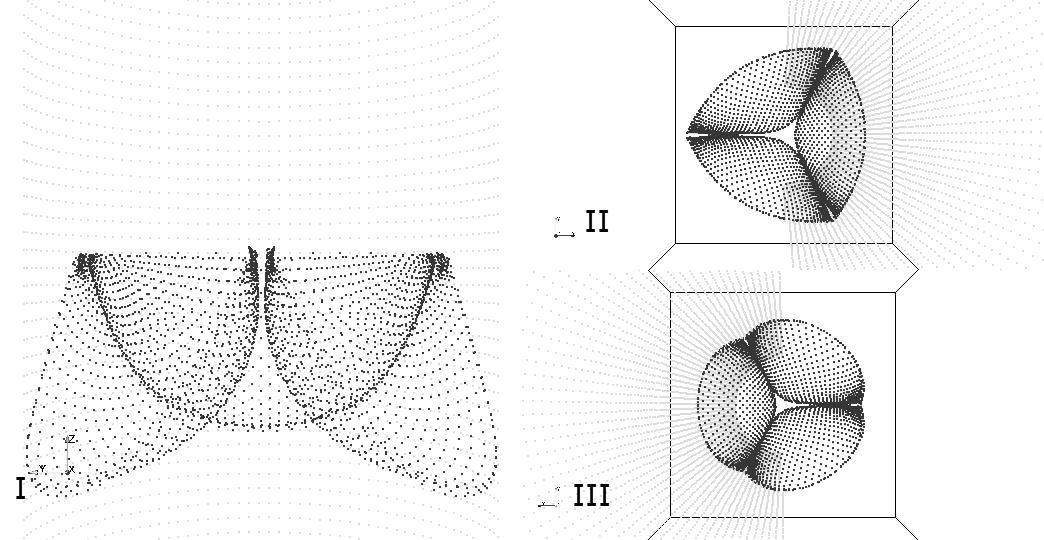
\includegraphics[height=6.2cm]{images/valve_1_gray.png}

$a$

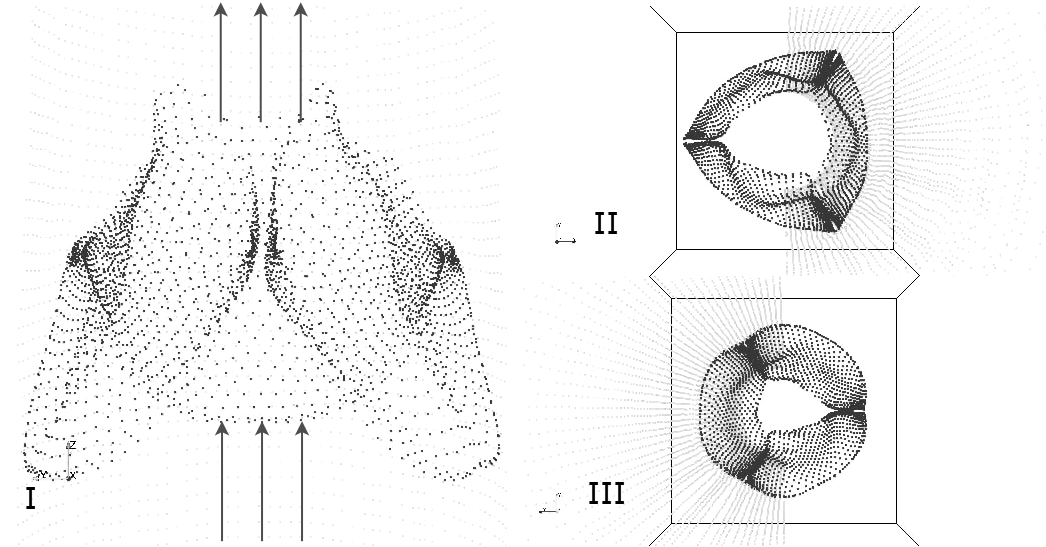
\includegraphics[height=6.2cm]{images/valve_2_gray.png}

$b$

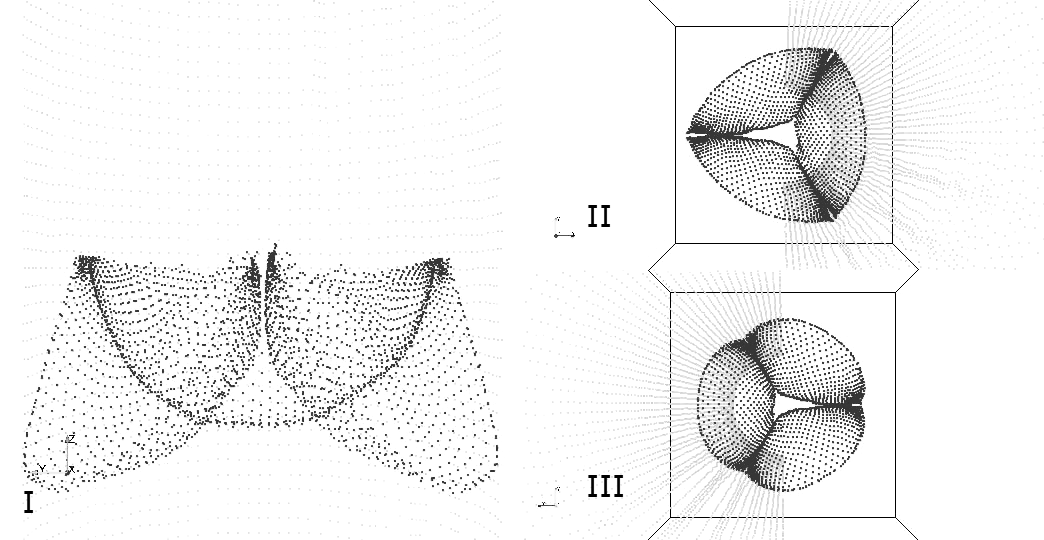
\includegraphics[height=6.2cm]{images/valve_3_gray.png}

$c$

\caption{Dynamics of the Valve leaflets. Current leaflet shape is indicated by points, arrows indicate flow direction.
Side view (I), front view (II) and rear view (III). $k_s = 5 \cdot 10^3$, $k_b = 5 \cdot 10^3$, $\rho_1 = \rho_2 = 1$,
$\mu_1 = \mu_2 = 1 \cdot 10^{-2}$; a) $t=0$, b) $t=0.7$, c) $t=1.5$}
\label{fig:valve}
\end{figure}

\begin{figure}
\centering
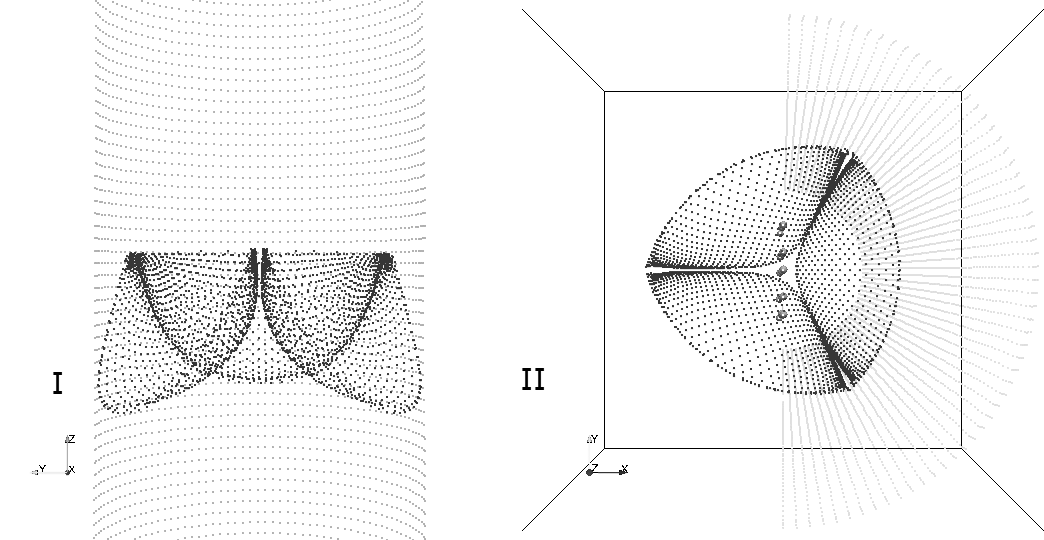
\includegraphics[height=6.2cm]{images/valve_with_particles_1_gray.png}

$a$

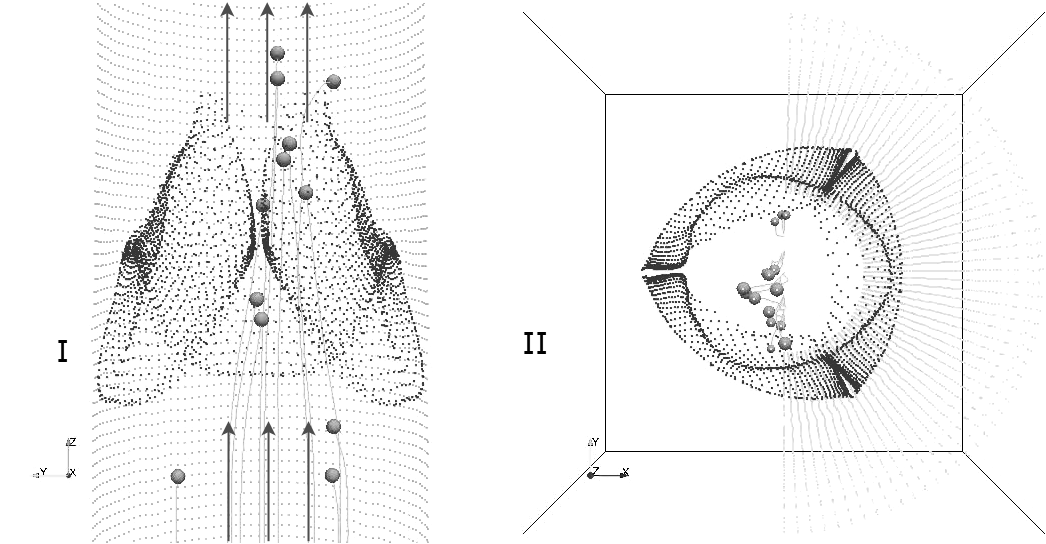
\includegraphics[height=6.2cm]{images/valve_with_particles_2_gray.png}

$b$

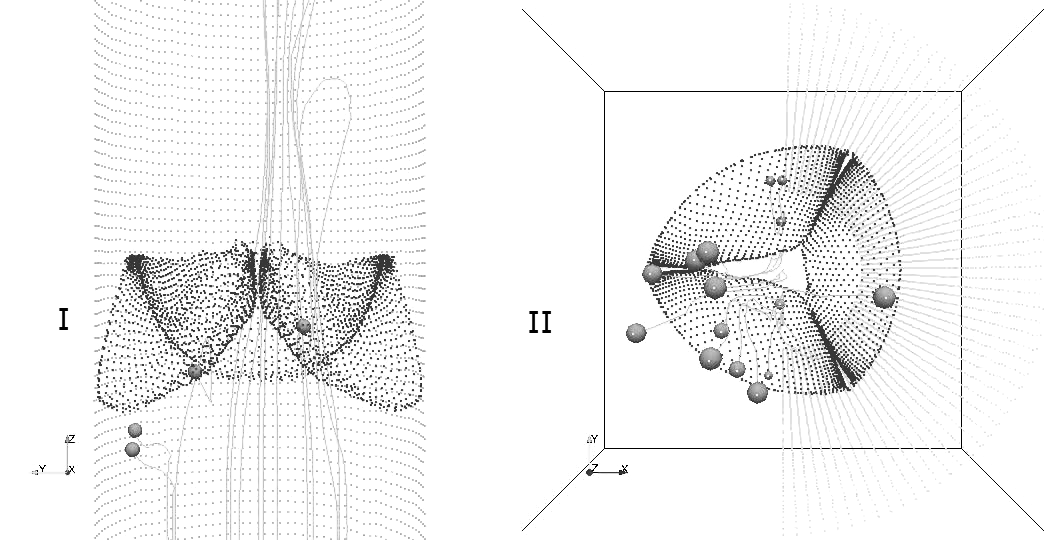
\includegraphics[height=6.2cm]{images/valve_with_particles_3_gray.png}

$c$

\caption{Tracks of particles inside the valve. Flow direction is indicated by arrows. Calculation parameters are the same as in the Fig. \ref{fig:valve}
Side view (I) and front view (II). $k_s = 5 \cdot 10^3$, $k_b = 5 \cdot 10^3$, $\rho_1 = \rho_2 = 1$,
$\mu_1 = \mu_2 = 1 \cdot 10^{-2}$; a) $t=0$, b) $t=0.7$, c) $t=1.5$}

\label{fig:valve_with_particles}
\end{figure}

As can be seen in the Fig. \ref{fig:valve} and Fig. \ref{fig:valve_with_particles}, the valve opens when pressure differential is increased,
and then reverts to the original state when pressure is balanced.

The Fig. \ref{fig:valve_in_mixture} shows the motion dynamics of the tricuspid valve under the pressure of fluid with variable viscosity and
density. Pressure differential $p_{in} - p_{out}$ changes cyclically from 0 to 6. Coefficient of stretching resistance $k_s = 8 \cdot 10^3$ and coefficient of
bending resistance $k_s = 6 \cdot 10^3$ are specified for the valve leaflets. Constant admixture flow with concentration $c_s = 0.45$ is set at $\Gamma_2$.

\begin{figure}
\centering
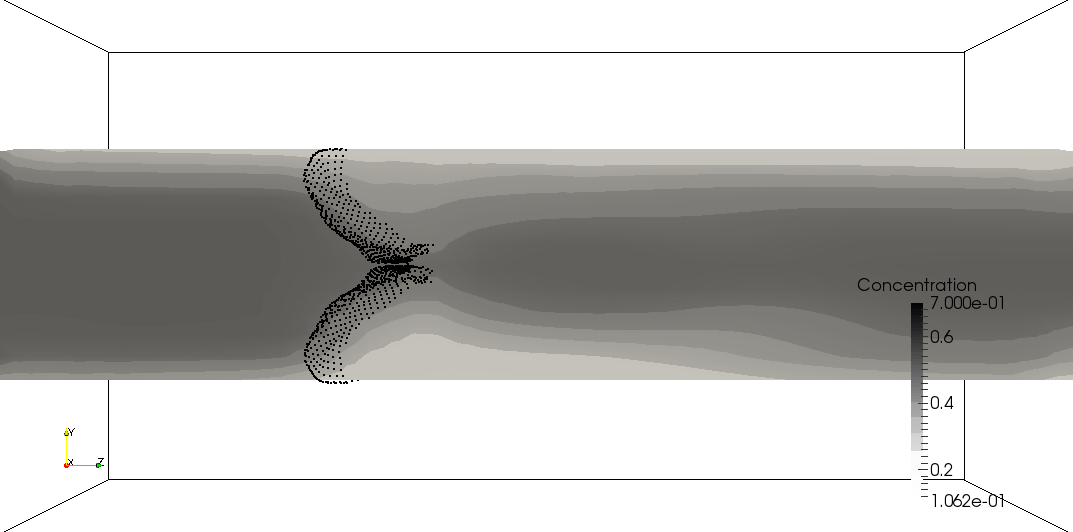
\includegraphics[height=6.2cm]{images/valves_in_mixture_gray_scale_400.png}

$a$

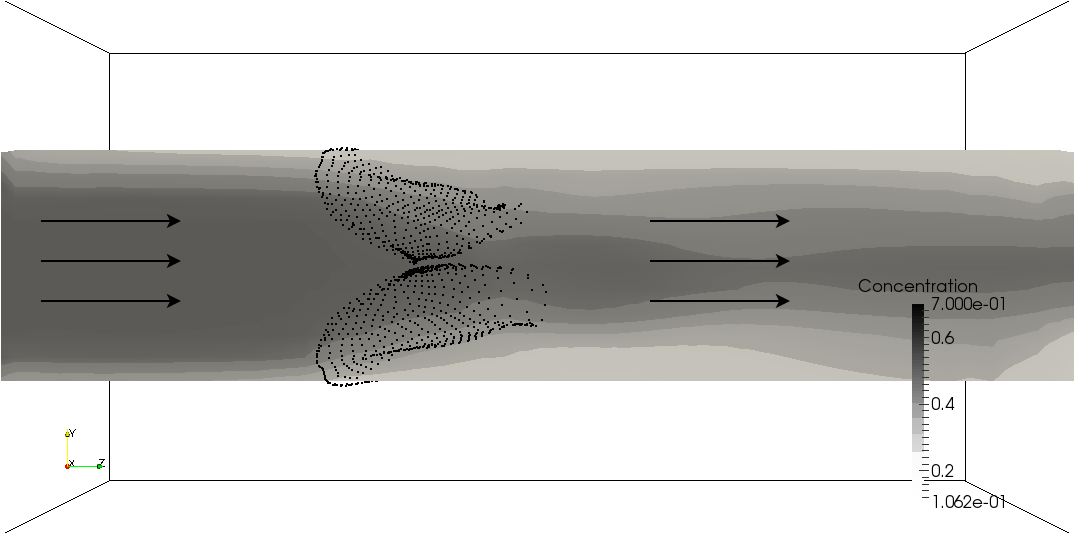
\includegraphics[height=6.2cm]{images/valves_in_mixture_gray_scale_500.png}

$b$

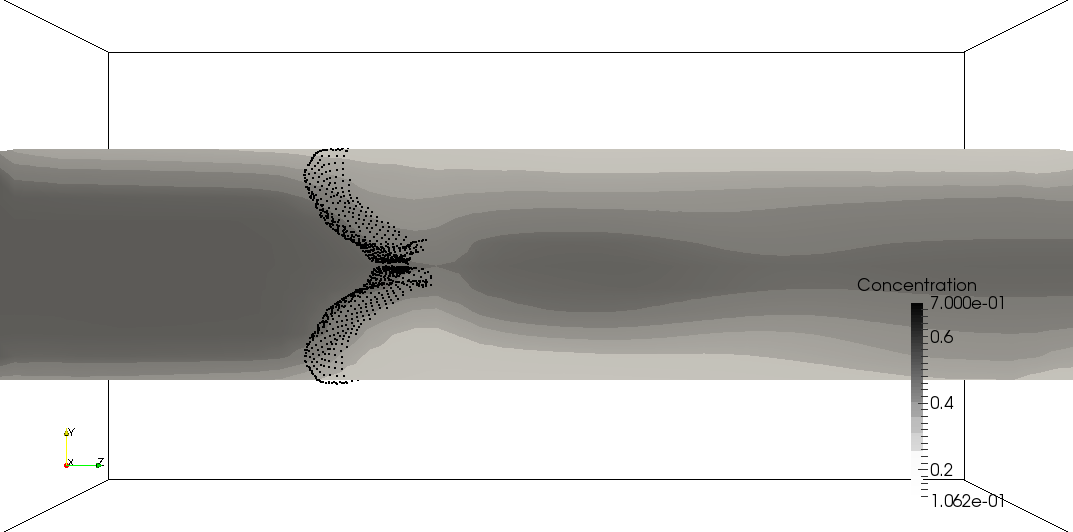
\includegraphics[height=6.2cm]{images/valves_in_mixture_gray_scale_600.png}

$c$

\caption{Valve leaflets motion in a vessel with variable viscosity and density. A constant admixture flow $c_s|_{\Gamma_2} = 0.45$ at the inflow,
admixture concentration at the initial time $c_0 = 0.45$, $\rho_1=1$, $\rho_2=1.2$, $\mu_1 = 1 \cdot 10^2$, $\mu_2 = 1.2 \cdot 10^2$;
a) $t = 4$, b) $t=5$, c) $t=6$}
\label{fig:valve_in_mixture}
\end{figure}

Fig. \ref{fig:valve_in_mixture} shows, that initial uniform admixture distribution is interrupted by the valve leaflets motion. Eventually oscillatory mode of
admixture motion can be recognized that corresponds to valve operating cycle. 
Moreover, the Fig. \ref{fig:valve_in_mixture} shows that admixture distribution over a cross section being parallel to axis $Oy$
is not symmetric because the valve leaflets are not symmetric about the axis $Oy$ as well.

\section{Conclusion}

Constructed model of blood flow with variable viscosity and density allows to get the patterns of leaflet deformation and admixture distribution 
effected by inhomogeneous fluid flow.

\begin{thebibliography}{4}

\bibitem{yoganathan} Yoganathan A.P., He Z.M., Jones S.C.: Fluid mechanics of heart valves. Annu. Rev. Biomed Eng 6:331--362 (2004)

\bibitem{yacoub} Yacoub N, Takkenberg J.: Will heart valve tissue engineering change the world? Nat Clin Prac Cardiovas Med. 2:60--1 (2005)

\bibitem{taylor} Taylor C.A., Hughes T.J.R., Zarins C.K.: Finite Element Modeling of Blood Flow in Arteries.
Computer Methods in Applied Mechanics and Engineering, vol. 158, 155--196, (1998)

\bibitem{zhang} Zhang Y, Bajaj C.: Finite element meshing for cardiac analysis. ICES Technical Report, 4--26 (2004)

\bibitem{black} Black M.M., Howard I.C., Huang X., Patterson E.A.: A three-dimensional analysis of a bioprosthetic heart valve. J. Biomech 24(9), 793--801 (1991)

\bibitem{pescin_1977} Peskin C.S.: Numerical Analysis of Blood Flow in the Heart. JCP 25, 220--252 (1977)

\bibitem{boyce_2011} Boyce E.G.: Immersed boundary model of aortic heart valve dynamics with physiological driving and loading conditions. International Journal for Numerical Methods in Biomedical Engineering. 1-29 (2011)

\bibitem{ma_x_2013} Ma X., Gao H., Boyce E.G., Berry C., Luo X.: Image-based fluid–structure interaction model of the human mitral valve. Computers \& Fluids 71, 417–425 (2013)

\bibitem{pilhwa_2010} Pilhwa L., Boyce E.G., Peskin C.S.: The immersed boundary method for advection-electrodiffusion with implicit time stepping and local mesh refinement. Comput Phys. 229(13), (2010)

\bibitem{fai_2013} Fai T.G., Boyce E.G., Mori Y., Peskin C.S.: Immersed boundary method for variable viscosity and variable density problems using fast constant-coefficient linear solvers I: Numerical method and results. SIAM Journal on Scientific Computing, 35(5), B1132–B1161, (2013)

\bibitem{jian} Jian D., Robert D.G., Aaron L.F., An immersed boundary method for two fluid mixtures// Journal of Computational Physics, Volume 262, 231--243, (2014)

\bibitem{lee} Lee P., Boyce E.G., Peskin C.S.: The immersed boundary method for advection-electrodiffusion with implicit time stepping and local mesh refinement. Journal of computational physics, Volume 229, 5208-5227, (2010)

\bibitem{gummel} Gummel E.E., Milosevic H., Ragulin V.V., Zakharov Y.N., Zimin A.I.: Motion of viscous inhomogeneous incompressible fluid of variable viscosity. Zbornik radova konferencije MIT 2013, Beograd, 267-274 (2014)

\bibitem{geidarov} Geidarov N.A., Zakharov Y. N.,  Shokin Yi. I.: Solution of the problem of viscous fluid flow with a given pressure differential. Russian Journal of Numerical Analysis and Mathematical Modeling, V.26, No 1, pp. 39--48 (2011)

\bibitem{milosevic} Milosevic H., Gaydarov N. A., Zakharov Y. N.: Model of incompressible viscous fluid flow driven by  pressure difference in a given channel. International Journal of Heat and Mass Transfer, vol. 62, July 2013 ISSN: 0017-9310, pp. 242--246, (2013)

\bibitem{dolgov} Dolgov D. A., Zakharov Y. N.: Modeling of viscous inhomogeneous fluid flow in large blood vessels. Vestnik Kemerovo State University, 2 (62) T.1, pp. 30--35 (2015)

\bibitem{caro} Caro C. G., Pedley Т. J., Schroter R. C., Seed W. A. The Mechanics of the Circulation. Moscow: Mir, p. 624 (1981)

\bibitem{ragulin} Ragulin V.V. To the problem of flow viscous fluid through the limited area under given pressure differential. Dynamic of continuum: Novosibirsk, Vol 27. p. 78--92 (1976)

\bibitem{pescin_2002} Peskin, C. S.: The immersed boundary method. Acta Numerica 11, 479–517 (2002).

\bibitem{goldstain} Goldstein D., Handler R., Sirovich L.: Modeling a no-slip flow boundary with an external force field. Journal of computational physics, 105, 354-366 (1993)

\bibitem{belotserkovsky} Belotserkovskii O. M.: Numerical modeling in mechanics of continuum. Moscow: Science, p. 520 (1984)

\bibitem{yanenko} Yanenko N. N.: Method of fractional steps for solving multidimensional problems of mathematical physics. Novosibirsk: Science, p. 197 (1967)

\end{thebibliography}

\end{document}
